\chapter{Développement d'application}

Comme présenté dans l'introduction (chapitre ~\ref{chap:intro}), le premier objectif du stage était le développement d'applications de réalité augmentée spatiale. Il était important, pour commencer, d'évaluer les possibilités mais aussi les contraintes qu'offrait le kit de développement. 
Ainsi, un travail d'analyse et de critique de l'API à été effectué en parallèle du développement d'applications.

\section{ReARTable}
\label{sec:reartable}
En tenant compte du contexte et du public ciblé par l'entreprise, il m'a paru intéressant de développer une démonstration dont le but était à la fois ludique et éducatif. J'ai donc choisi de recréer une Reactable\cite{reactable}, proposée par la société du même nom, en réalité augmentée spatiale, appelée ReARTable.

La Reactable est un instrument de musique électronique permettant la génération de sons en direct, développé depuis 2003. Présenté sous la forme d'une table interactive, le son est généré via des éléments tangibles placés à sa surface Figure~\ref{fig:reactelem}. 

\begin{figure}[H]
\centering
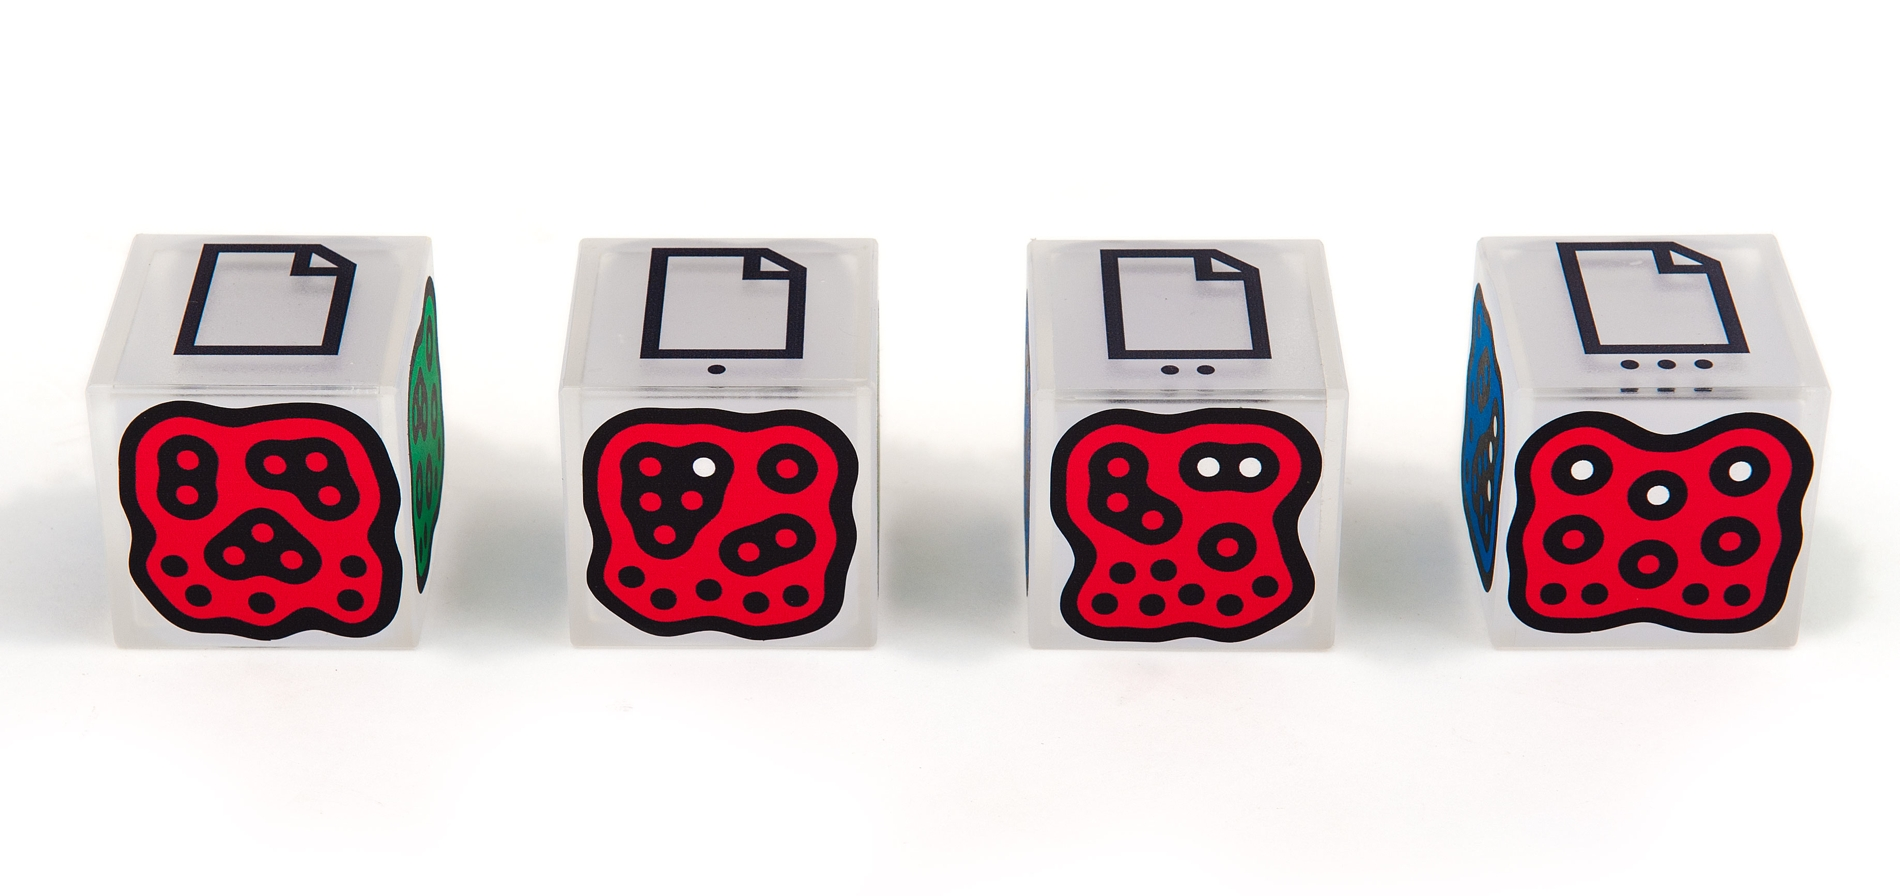
\includegraphics[width=0.6\textwidth]{images/reactelements}
\caption{Éléments tangibles utilisés pour la génération d'un élément de synthétiseur sur la Reactable\protect\footnotemark}
\label{fig:reactelem}
\end{figure}

\footnotetext{Source: \href{http://a-blok.com/FR/reactable.html}{Reactable : Elements tangibles}}

Chaque élément tangible représente un élément de synthétiseur qu'il est possible de contrôler de plusieurs façons:
\begin{itemize} 
\item La distance de l'élément par rapport à un autre élément. Cette propriété peut être utilisée pour contrôler, par exemple, l'interaction entre deux éléments.
\item L'orientation de l'élément sur la table. Cette propriété peut être utilisée pour contrôler, par exemple, la fréquence de l'élément ce qui va avoir pour effet si l'on prend l'exemple d'un battement de ralentir ou d'accélérer ce dernier.
\item La disposition de l'élément. Cette propriété permet, entre autres, de combiner des éléments pour créer de nouveaux sons, plus riches et plus complexes.
\item La position du doigt de l'utilisateur par rapport à un élément. On peut venir contrôler divers paramètres comme l'amplitude par exemple, en faisant graviter son doigt autour d'un élément.
\end{itemize}
Ainsi, c'est en combinant plusieurs éléments entre eux avec différentes orientations et différentes dispositions que l'utilisateur va pouvoir peu à peu "construire" sa musique.
Au-delà de la détection des éléments tangibles, la table est rétro éclairée et permet donc la visualisation, en direct, de la musique générée Figure~\ref{fig:reactivsu}.

\begin{figure}[H]
\centering
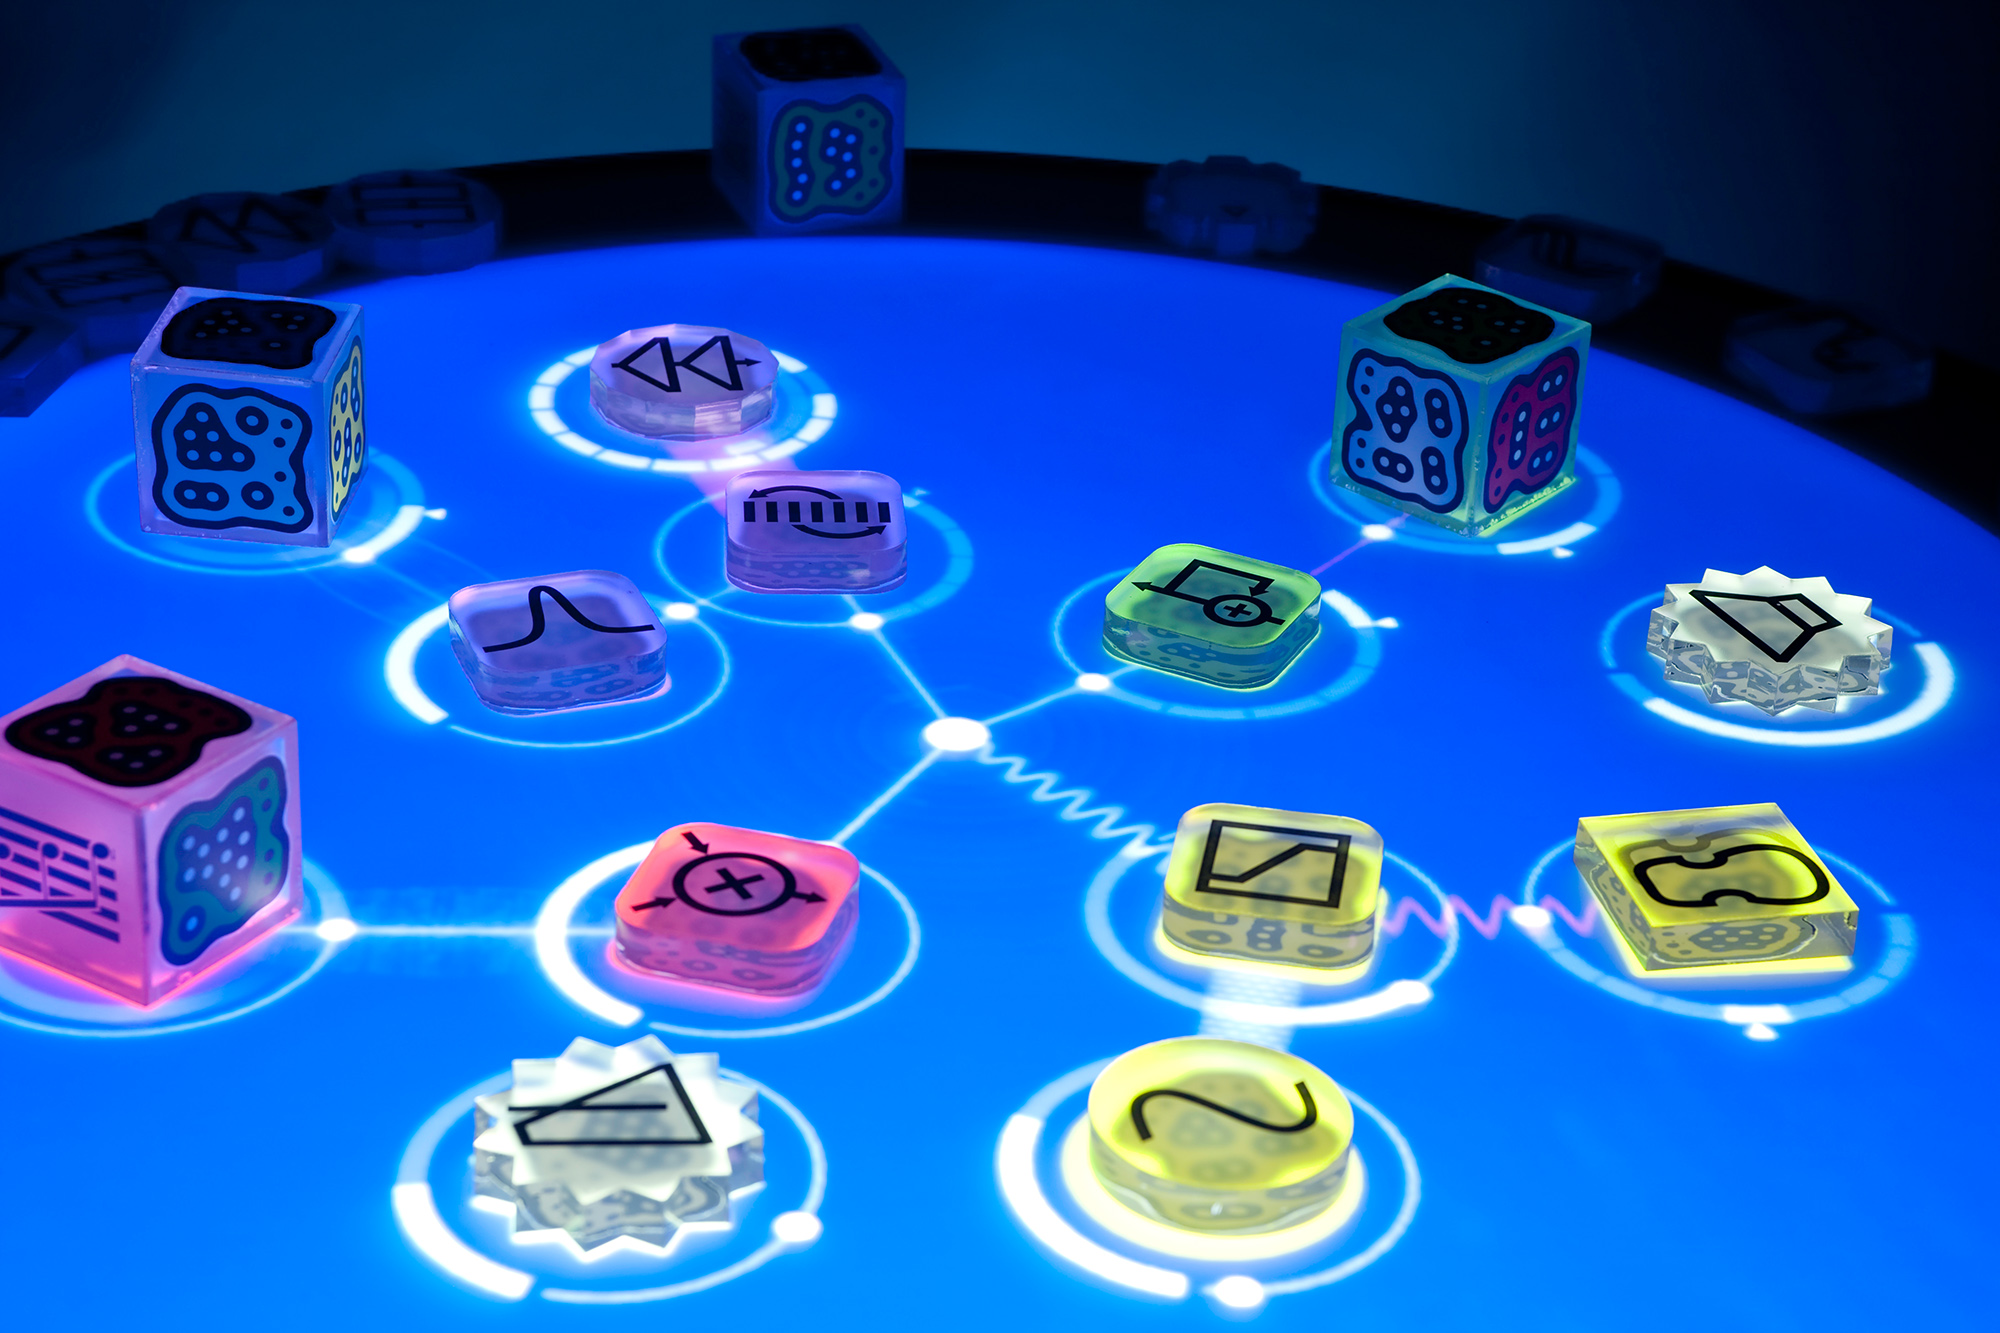
\includegraphics[width=0.65\textwidth]{images/reactvisu}
\caption{Visualisation du son sur la Reactable\protect\footnotemark}
\label{fig:reactivsu}
\end{figure}

\footnotetext{Source: \href{http://a-blok.com/FR/reactable.html}{Reactable}}

\subsection{Besoins de l'application}
\label{subsec:reartable:content}
Le but de l'application était de présenter une démonstration de ce qu'est capable de faire le système proposé par RealityTech, et non de créer un simulateur de musique en direct, finit, reprenant tous les points de la Reactable. Un tel développement pourrait faire l'objet d'un stage entier, ce qui n'était pas le cas ici.\\

Pour être en adéquation avec l'idéologie de l'entreprise, l'interface tangible ainsi que les modes d'interaction avec la musique étaient les points les plus importants à considérer. En gardant cela à l'esprit, nous avons défini les besoins fonctionnels principaux que voici :
\begin{itemize}
\item Générer du son en direct.
\item Créer une représentation physique du son. Chaque son ou élément sonore devait avoir une représentation physique qui lui était associée, c'est à dire, un élément ou groupement d'éléments tangibles représentant ce son.
\item Détecter des éléments physiques représentant les éléments sonores dans une image. L'application devait pouvoir détecter dans une image de caméra les divers éléments physiques présents, de façon à ce qu'ils soient utilisés pour identifier les éléments sonores.
\item Identifier les représentations physiques des sons. Chaque élément sonore étant représenté par un ou plusieurs éléments physiques, l'application devait être capable, à partir des résultats de la détection, d'identifier et de différencier des éléments sonores entre eux. 
\item Modifier un élément sonore. L'application devait pouvoir contrôler certains paramètres définis à l'avance de chaque élément sonore généré. Ces paramètres ont pour but d'apporter à l'utilisateur un niveau de contrôle supérieur lors de la création de musique en direct.
\item Détecter des événements liés au toucher. Dans le cas du contrôle d'un son, l'utilisateur peut être amené à toucher des zones interactives pour déclencher divers effets.
\item Créer une visualisation basique d'un son. L'application devait proposer une visualisation du son généré, pour guider l'utilisateur dans son expérimentation.
\end{itemize}

\subsection{Choix et implémentation}
\label{subsec:reartable:impl}
L'application a donc été développée avec Processing, en utilisant, d'une part, PapARt pour la partie visualisation, détection et projection et, d'autre part, Sonic Pi\cite{sonicpi} pour la génération de musique en direct.
Sonic Pi est un synthétiseur temps réel qui permet de générer très facilement des sons de manière cohérente. Le gros avantage de Sonic Pi est qu'il résout tout seul bon nombre de problèmes posés par la génération dynamique de musique comme, par exemple, la synchronisation des boucles, les effets d'entrée et de sortie des instruments et bien d'autres, ce qui dé-complexifie énormément le processus.

Comme on peut le voir sur le schéma explicatif ci-dessous Figure~\ref{fig:reartable:generalscheme}, les éléments tangibles représentant des sons apparaissent sous forme de regroupement d'éléments ronds de petite taille (des aimants dans notre cas). L'idée derrière ce choix est d'encourager la manipulation d'éléments physiques pour garder le contenu numérique en contexte et ainsi favoriser la création. On peut différencier deux sons en fonction du contenu du regroupement (nombre, position et couleur des éléments regroupés).

\begin{figure}[H]
\centering
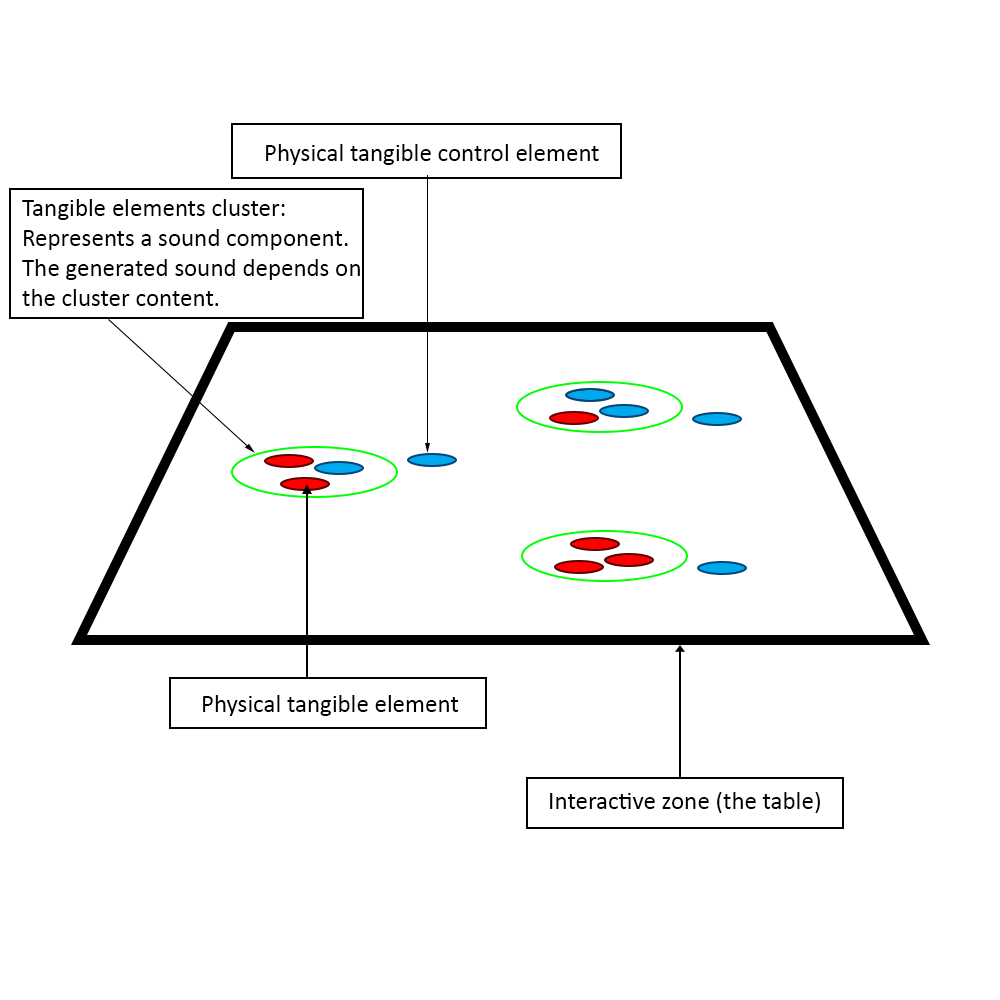
\includegraphics[width=0.5\linewidth]{images/rearproto}
\caption{ReARTable: Illustration du concept}
\label{fig:reartable:generalscheme}
\end{figure}

Une fois les éléments détectés, regroupés et identifiés, l'élément sonore associé peut être créé. La création de l'élément sonore se fait simplement via la transmission d'un message OSC\footnote{Le protocole OSC ou OpenSoundControl est un format de transmission de donnée conçu pour le contrôle en temps réel} à un serveur Sonic Pi préalablement démarré. Ce message contient l'identifiant unique de la boucle que Sonic Pi doit démarrer. Pour chaque élément sonore que l'application peut créer, Sonic Pi possède une fonction à exécuter que nous avons préalablement créée. Toutes les communications entre l'application et Sonic Pi utilisent ce protocole ce qui permet de démarrer/arrêter/modifier certaines parties du son en direct.

Pour ce qui est du contrôle du son, une zone autour du composant est définie dans laquelle soit un élément tangible, soit une interaction physique (avec le doigt) vont être détectés et convertis en interaction avec le contenu numérique Figure~\ref{fig:reartable:interactionzone}.

\begin{figure}[H]
\centering
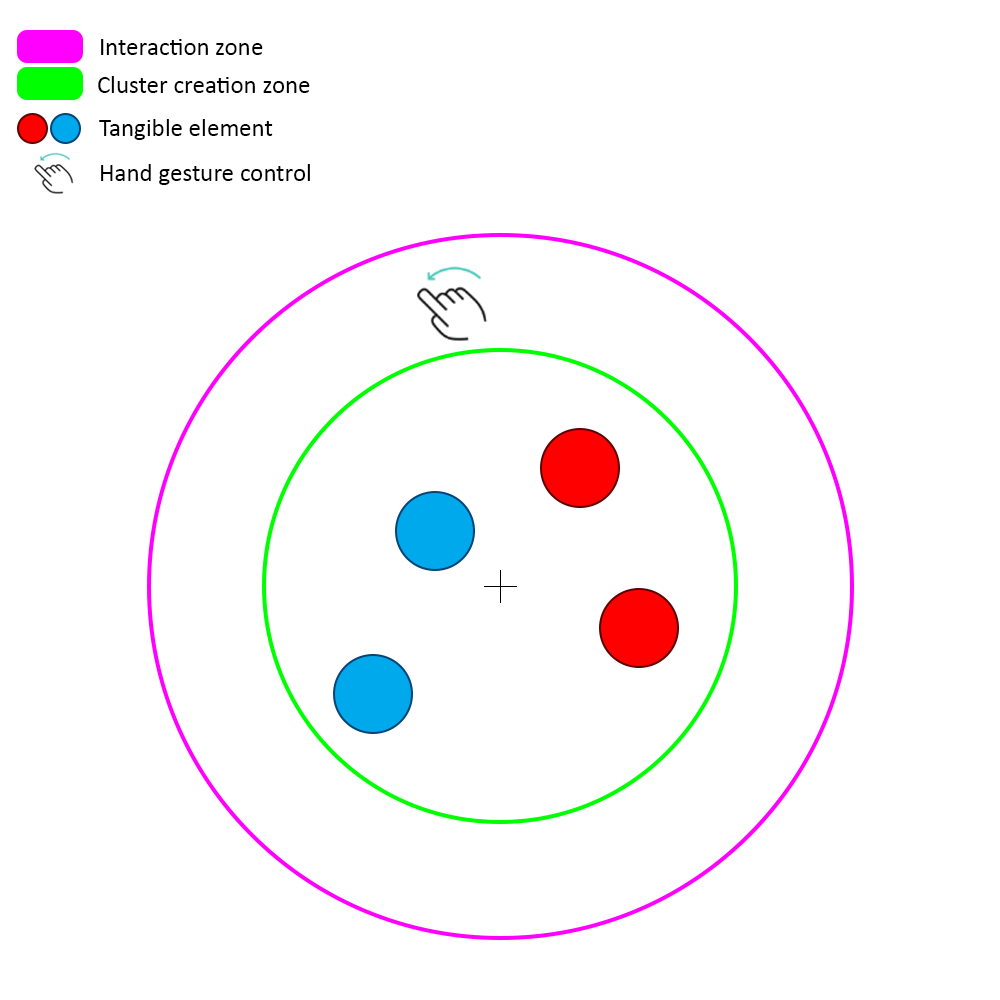
\includegraphics[width=0.45\textwidth]{images/reartable_cluster_interaction}
\caption{Schéma représentant la création d'un son avec zone d'interaction}
\label{fig:reartable:interactionzone}
\end{figure}

La dernière étape du développement de l'application concernait la visualisation de la musique générée section~\ref{subsec:reartable:content}. Cette étape n'a finalement pas été aboutie par manque de temps. L'idée était d'utiliser le spectre du son et les différentes fréquences qui le compose, récupérables à l'aide d'une transformée de Fourier\footnote{Opération mathématique permettant de décomposer un signal en la somme des signaux qui le compose \href{https://fr.wikipedia.org/wiki/Transformation_de_Fourier}{Wikipédia - Transformation de Fourier}.}, pour créer une visualisation globale basée sur les fréquences avec des variations visuelles en fonction de la hauteur, du tempo du son et de tous les autres paramètres du son que l'on peut extraire.\\

Vous trouverez Figure~\ref{fig:reartable:demo} un aperçu de l'état actuel de l'application. 

\begin{figure}[H]
\centering
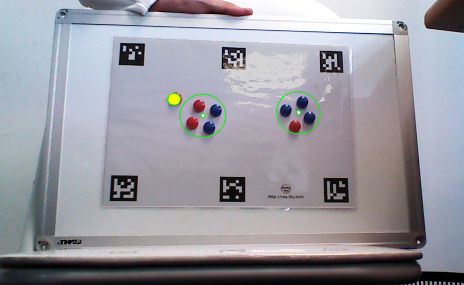
\includegraphics[width=0.65\linewidth]{images/reartable}
\caption{Démonstration de l'application}
\label{fig:reartable:demo}
\end{figure}

\newpage
\section{Extraction de document}
\label{sec:document}
Plus tard au cours de mon stage, nous avons eu l'occasion d'aborder des problématiques comme l'extraction et la numérisation de document (par exemple dans le cas de l'écriture d'une lettre en réalité augmentée) en tant que cas d'utilisation de PapARt. Il était donc opportun de développer une preuve de concept de cette fonctionnalité sous la forme d'une application de SAR.

Le but de ce développement était d'expérimenter diverses techniques de détection de document en temps réel, se basant ou non sur des connaissances à priori comme la taille du document, sa couleur, la couleur du fond (duquel il faudrait extraire le document), la présence d'éléments distinctifs (tels que des marqueurs fiduciaires ou des ronds colorés de petite taille) etc.

\subsection{Besoins de l'application}
\label{subsec:doc:content}
\begin{itemize}
\item Accéder au flux vidéo d'une caméra. L'application devait avoir access au flux vidéo d'une caméra filmant le document à détecter.
\item Détecter un document dans une image. Des images extraites du flux vidéo, l'application devait être capable, avec ou sans connaissance a priori, de détecter un document se trouvant dans cette image.
\item Extraire un document d'une image. Grâce au résultat de la détection, l'application devait être capable d'extraire ce document de l'image afin d'obtenir une image ne contenant que le dit document.
\end{itemize}

\subsection{Choix et implémentation}
\label{subsec:doc:impl}

La détection de document est un problème connu en traitement d'image, sur lequel j'avais déjà eu l'occasion de travailler lors de mon projet de fin d'études durant le deuxième semestre de mon année de Master 2.

Dans cette application, nous avons mis en place plusieurs détections différentes pour essayer de trouver une solution à ce problème.

\subsubsection{Détection de document basée sur des marqueurs colorés} Le premier prototype de détection utilise une connaissance à priori sur le document: Le document cible est muni de lignes d'éléments ronds, colorés, de petite taille, dans un ou plusieurs de ses coins (fig~\ref{sub:doc}). Les éléments ronds de petite taille sont détectés grâce à PapARt en réalisant une convolution de l'image par un filtre permettant la détection de ces derniers.

Une fois les éléments détectés, ils sont regroupés en différentes lignes (fig~\ref{sub:doc:line}).
Une ligne est définie par un regroupement d'éléments dont l'écart entre chaque élément ne dépasse pas une certaine distance verticale ou horizontale. L'angle de la ligne est défini par les $x$ premiers éléments qui la compose, $x$ étant le nombre minimum d'éléments composant une ligne (fig~\ref{fig:doc:linecluster}). Si un autre élément "dérive" il est rejeté et la ligne est créée. Cette ligne est ensuite utilisée pour calculer deux vecteurs, dont un est confondu avec la ligne et le deuxième est perpendiculaire au premier (fig~\ref{sub:doclineperp}).

La détection finale du document se fait en calculant l'intersection des différents vecteurs verticaux et horizontaux (fig~\ref{sub:docextract})

\begin{figure}[H]
    \centering
	\subfloat[Document marqué à détecter]{
      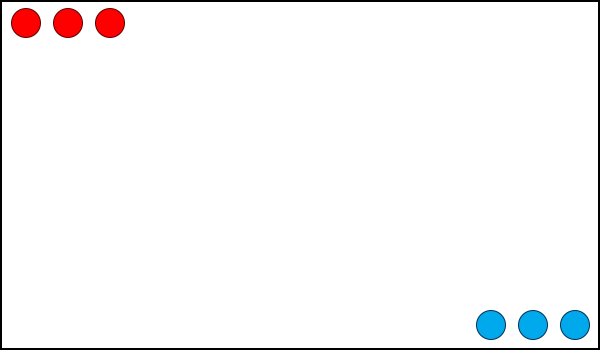
\includegraphics[width=0.45\textwidth]{images/document}
      \label{sub:doc}
      }
    \subfloat[Détection des éléments rond et création des lignes]{
      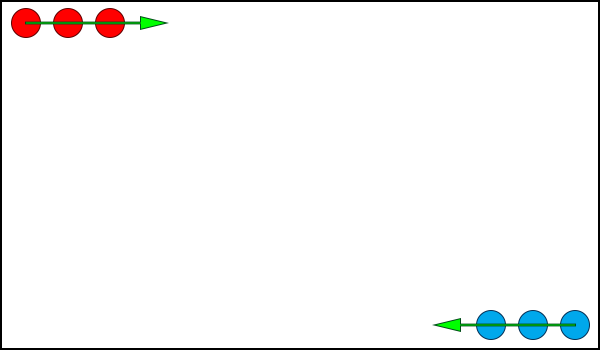
\includegraphics[width=0.45\textwidth]{images/doc-line}
      \label{sub:docline}
      }
      \\
      \subfloat[Génération des information manquante pour finaliser la détection]{
      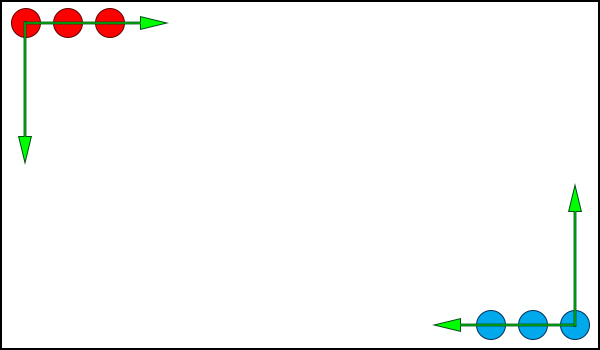
\includegraphics[width=0.45\textwidth]{images/doc-line-perp}
      \label{sub:doclineperp}
      }
    \subfloat[Document détecté]{
      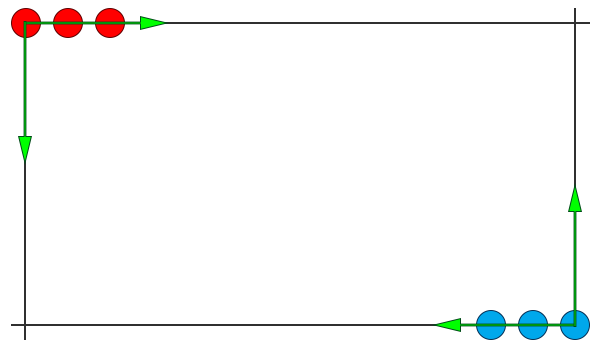
\includegraphics[width=0.45\textwidth]{images/doc-extraction}
      \label{sub:docextract}
      }
\caption{Détection de document étape par étape}
\label{fig:docdetection}
\end{figure}
	
\begin{figure}[H]
\centering
	\subfloat[]{
      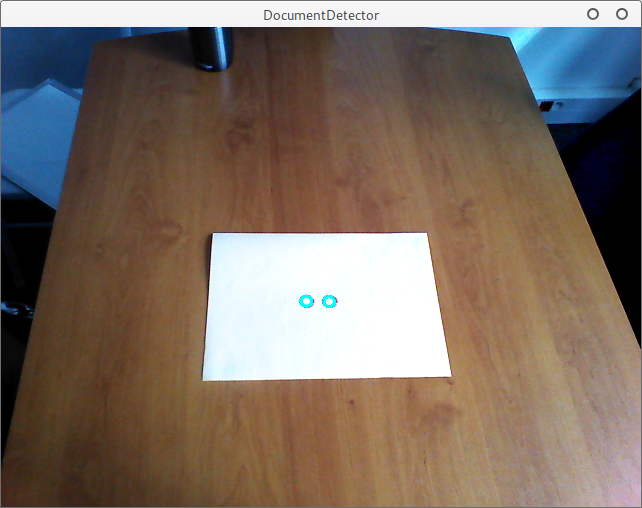
\includegraphics[width=0.45\textwidth]{images/document-detection-noline}
      \label{sub:doc:noline}
      }
      \subfloat[]{
      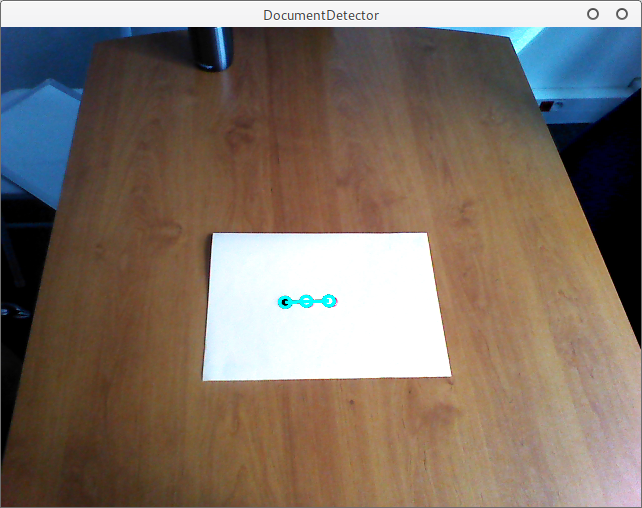
\includegraphics[width=0.45\textwidth]{images/document-detection-line}
      \label{sub:doc:line}
      }
      \caption{Détection et création d'une ligne a partir d'éléments colorés ($x = 3$)}
      \label{fig:doc:linecluster}
\end{figure}

Comme on peut le voir sur la figure ~\ref{sub:docextract}, lors de cette détection, les bords du document sont rognés. Généralement ces zones ne contiennent aucune information car elles correspondent le plus souvent aux marges verticales et horizontales présentes dans la plupart des documents. Cependant, comme évoqué dans les cas d'utilisation, cette détection ne sera pas seulement utilisée pour des documents de type A4, on pourra s'en servir comme outil pour suivre une feuille de papier à la manière des marqueurs ARToolKit, ou pour détecter des post-it par exemple. Ainsi, ces marges ne peuvent pas être ignorées car elle sont susceptibles de contenir du contenu critique du document.

Une simple connaissance à priori de la distance des éléments ronds par rapport au coin permet de résoudre ce problème. Toutefois, si l'on souhaite obtenir une détection plus précise, il est conseiller d'utiliser des algorithmes de détection de contour couplés à des algorithmes d'extraction de lignes qui permettrons de retrouver de façon plus fidèle le coin du document. Cette re détection du coin est détaillée section~\ref{subsubsec:cannyhough}.

\subsubsection{Détection de document - Canny et transformée de Hough}
\label{subsubsec:cannyhough} 
Sans connaissance à priori, la détection de document devient un problème compliqué et bien connu dans le domaine du traitement d'image surtout lorsqu'un besoin de temps réel vient s'ajouter à la tâche.

L'algorithme de Canny\cite{Canny86acomputational} est un filtre de détection de contours, permettant d'extraire d'une image des contours très précis (fig ~\ref{sub:detectedge}) respectant trois critères : La bonne détection, la bonne localisation et la clarté de la réponse. Ces trois critères en font un très bon choix dans le cadre de la détection de document, où la qualité et surtout la précision de la détection est importante pour ne pas rogner des bouts de document par exemple. Cet algorithme a cependant tendance à laisser beaucoup de bruit issu de faibles contours tout de même détectés. C'est pourquoi il faut effectuer une étape de floutage préalable afin de lisser les zones à faibles contours.

Une fois les contours détectés, il est possible d'essayer d'extraire directement le document mais c'est une tâche complexe car elle requiert d'analyser les contours. Cette action peut être facilitée en utilisant une technique appelée transformée de Hough\cite{hough}. En effet, la transformée de Hough permet d'extraire n'importe quelle forme à partir d'une image contour en utilisant les propriétés mathématiques de la forme. Dans notre cas, où nous souhaitons extraire des lignes droites, les propriétés mathématiques utilisées correspondent aux coordonnées polaires considérées comme plus robuste que l’équation de la droite (fig ~\ref{sub:detectline}). Il ne reste qu'à filtrer les lignes afin de trouver des potentiels documents dans une image.

\begin{figure}[H]
\centering
	\subfloat[Image originale]{
      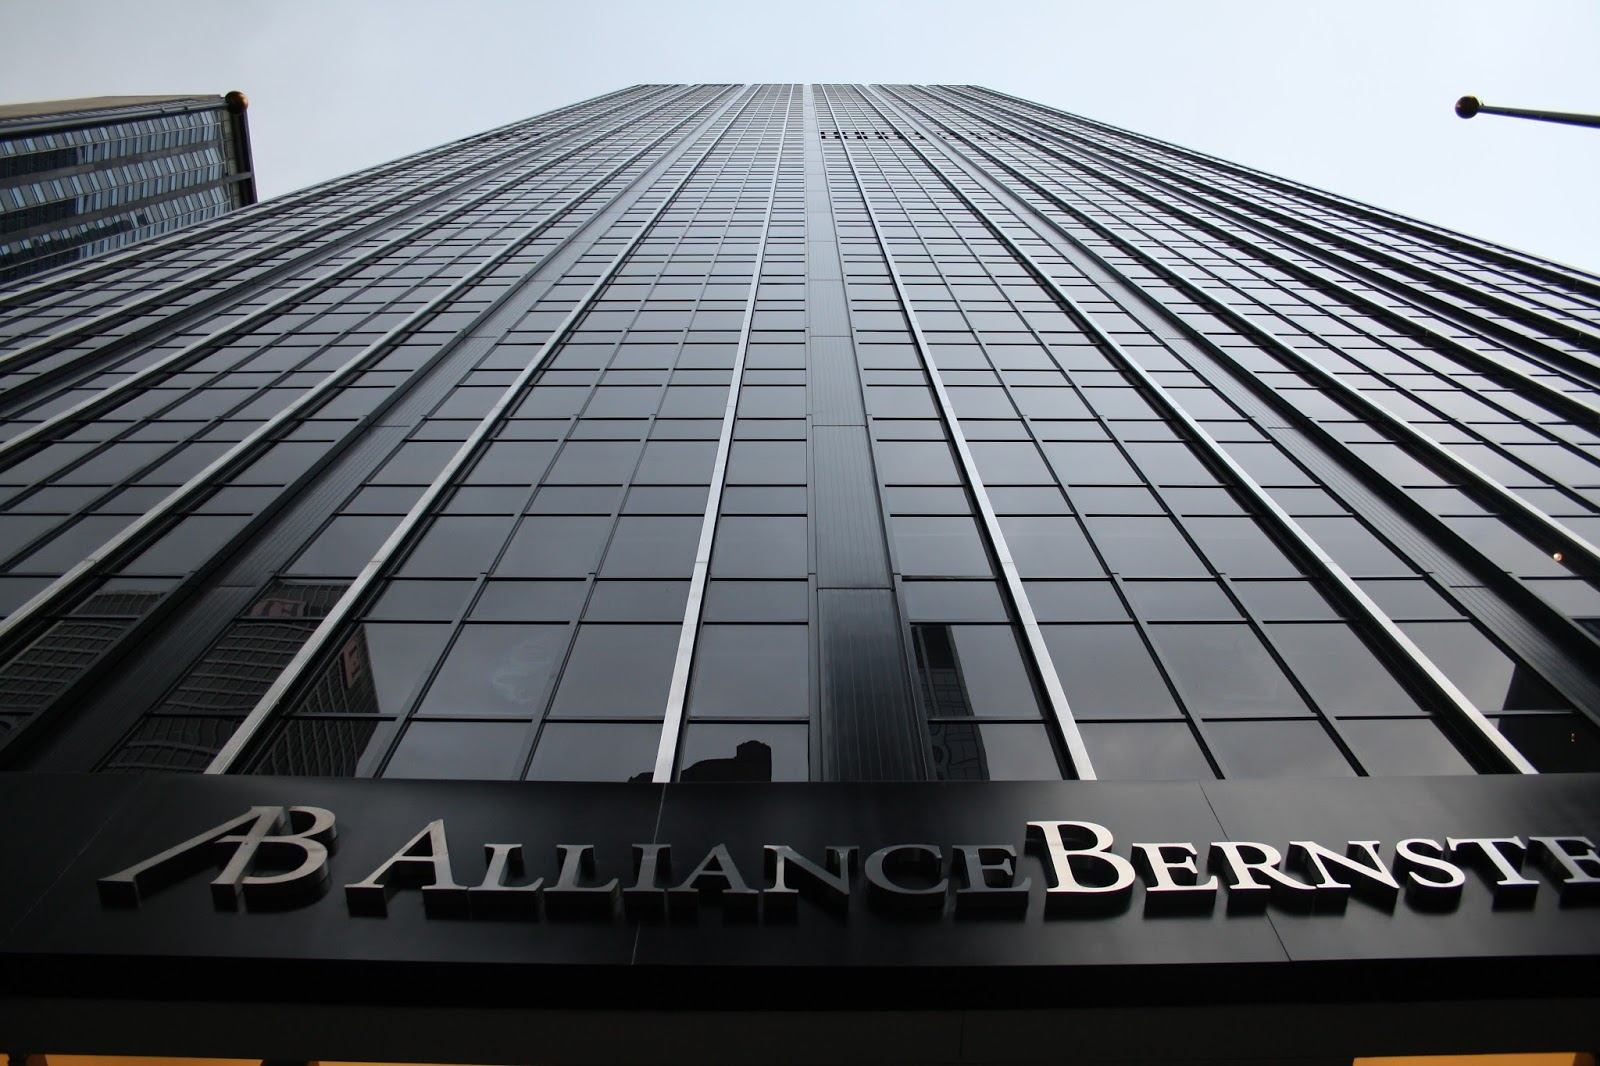
\includegraphics[width=0.45\textwidth]{images/detection-original-image}
      \label{sub:originalimage}
      }
      \\
	\subfloat[Canny - Détection de contours]{
      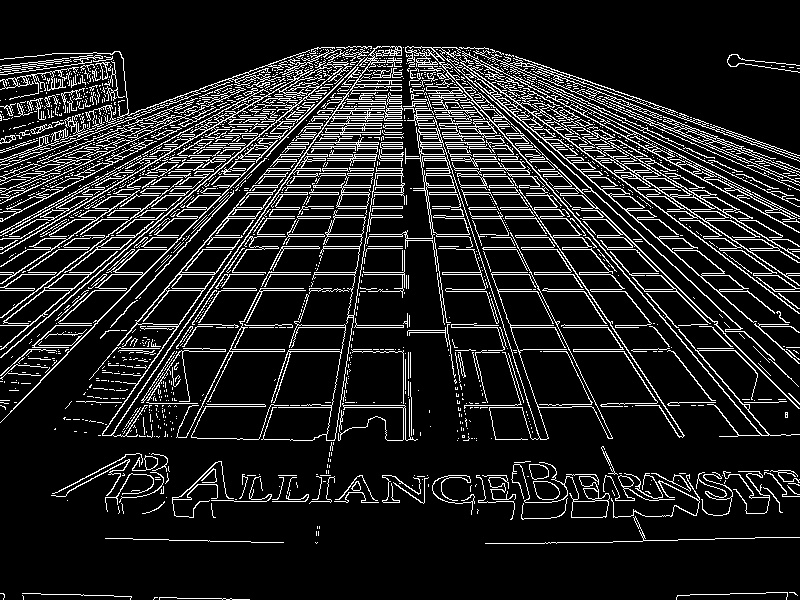
\includegraphics[width=0.45\textwidth]{images/cannysample}
      \label{sub:detectedge}
      }
    \subfloat[Transformée de Hough - Détection de lignes]{
      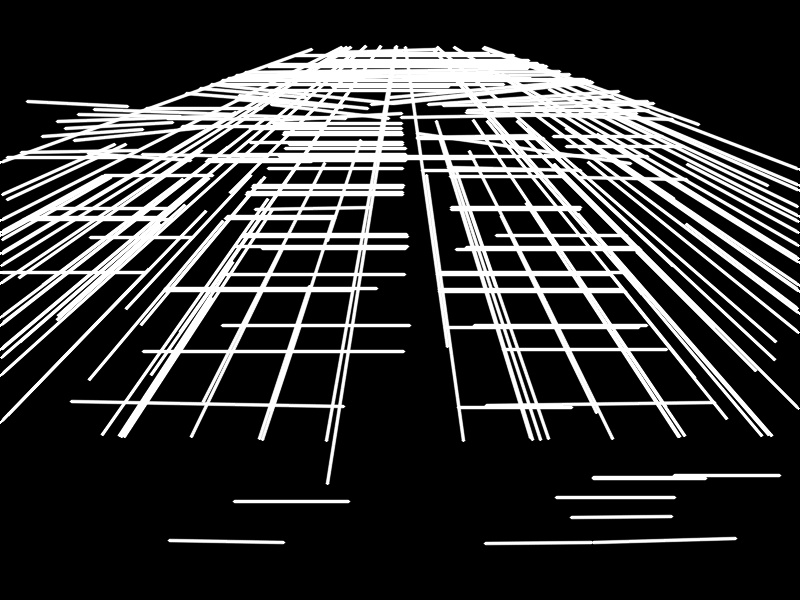
\includegraphics[width=0.45\textwidth]{images/houghsample}
      \label{sub:detectline}
      }
\caption{Détection de lignes : Canny + Hough\protect\footnotemark}
\label{fig:cannyhough}
\end{figure}
\footnotetext{Source : \href{http://funvision.blogspot.com/2016/01/hough-lines-and-canny-edge-sobel.html}{http://funvision.blogspot.com/2016/01/hough-lines-and-canny-edge-sobel.html}}

Cette succession de traitements est cependant lourde et peut difficilement être effectuée en temps réel sur des images haute résolution. 

Dans notre cas, nous nous somme servis de ces deux algorithmes mais uniquement sur des parties d'image (de petite résolution) de façon à améliorer une première détection grossière effectuée notamment à l'aide de marqueurs colorés. Une fois la première détection effectuée, nous obtenons une position plus ou moins précise des quatre coins nécessaires à l'extraction du document. Nous utilisons cette information sur la position potentielle des coins pour extraire des sous-images centrées sur ces coins (fig. ~\ref{sub:subimage:subimage}) que nous seuillons afin d'obtenir une image binaire Figure~\ref{sub:subimage:tresh}. Ensuite, nous appliquons les deux algorithmes mentionnés plus tôt, à savoir la détection de contours (fig. ~\ref{sub:subimage:canny}) puis la détection de lignes (fig. ~\ref{sub:subimage:hough}). Après cela, nous filtrons le résultat de la détection de ligne pour obtenir exactement une ligne verticale et une ligne horizontale. Une fois ces deux lignes trouvées, nous calculons les équations de droite (pente et constante) associées, pour pouvoir en calculer l'intersection et ainsi trouver le coin dans notre sous image (fig ~\ref{sub:subimage:corner}).

\begin{figure}[H]
\centering
	\subfloat[Sous image autour d'un coin.]{
      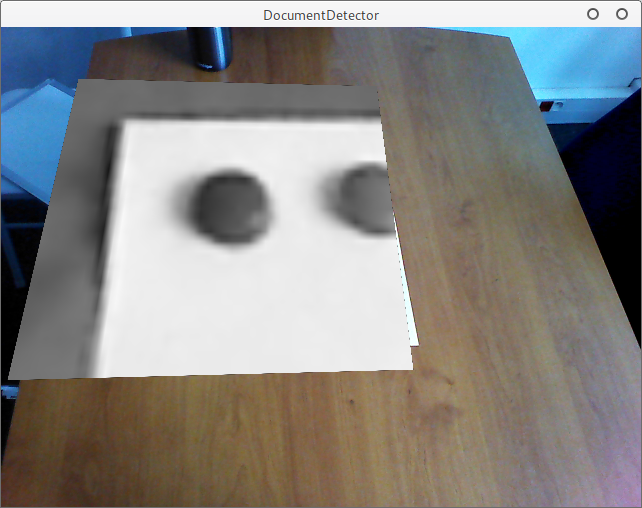
\includegraphics[width=0.33\textwidth]{images/doc-original}
      \label{sub:subimage:subimage}
      }\\
      \subfloat[Seuillage de l'image originale]{
      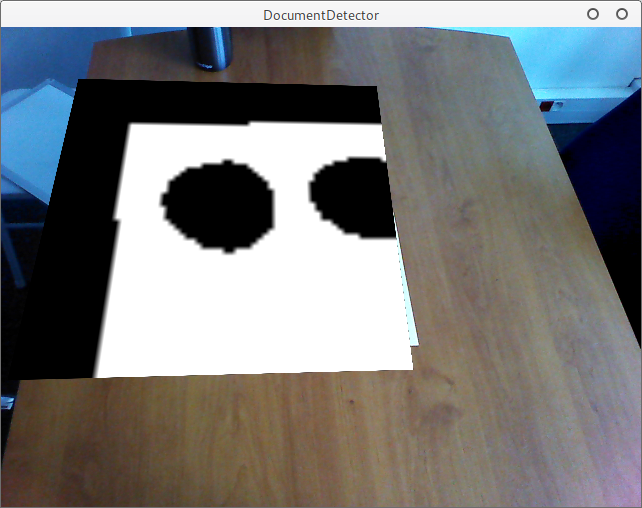
\includegraphics[width=0.33\textwidth]{images/doc-tresh}
      \label{sub:subimage:tresh}
      }
    \subfloat[Canny - Détection de contour basée sur un seuillage de l'image originale]{
      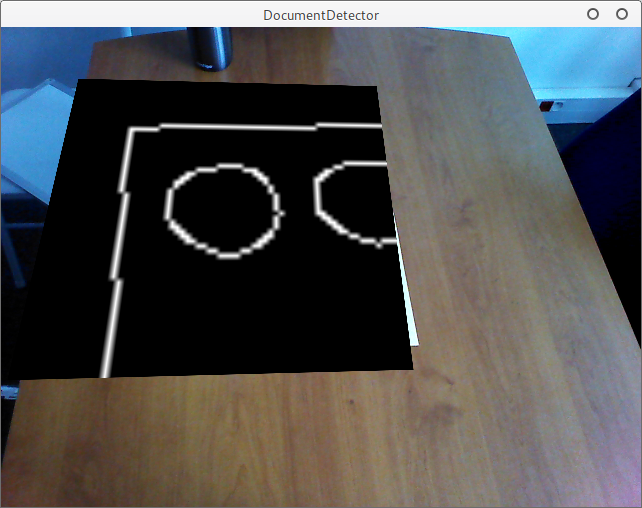
\includegraphics[width=0.33\textwidth]{images/doc-canny}
      \label{sub:subimage:canny}
      }
      \\
	\subfloat[Hough - Détection de lignes basée sur le résultat de Canny]{
      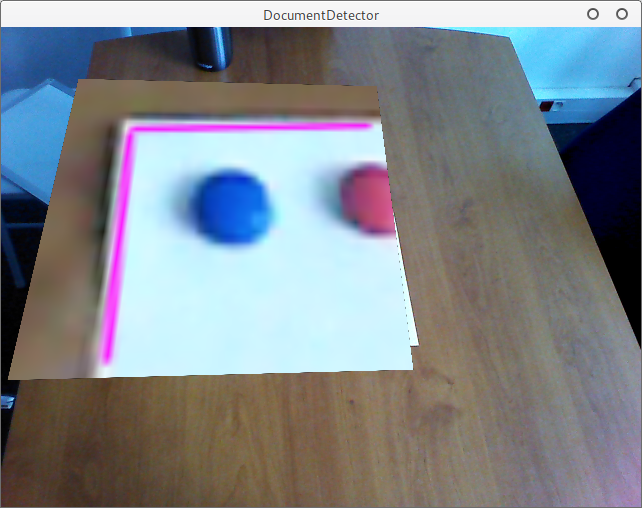
\includegraphics[width=0.33\textwidth]{images/doc-hough}
      \label{sub:subimage:hough}
      }
    \subfloat[Détection finale du coin.]{
      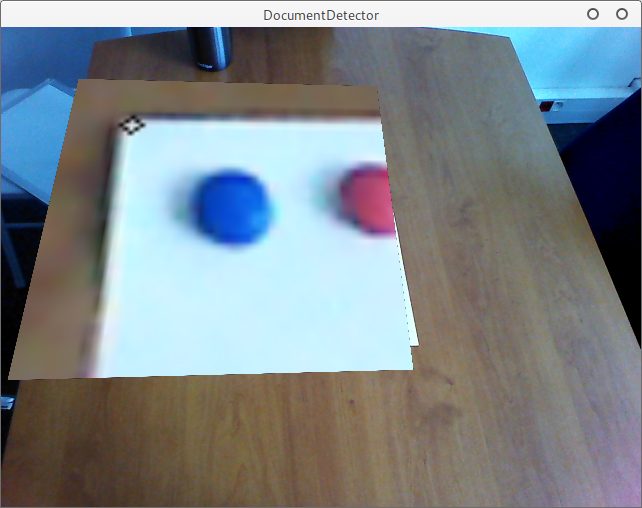
\includegraphics[width=0.33\textwidth]{images/doc-corner}
      \label{sub:subimage:corner}
      }
\caption{Affinage de la détection d'un coin du document}
\label{fig:corner-redetect}
\end{figure}

\subsection{Bilan}
\label{subsec:doc:bilan}
Pour finir, un comparatif des différents résultats obtenus est présenté sur la Figure~\ref{fig:docdetect:results}.
On peut observer quelques points notables : En utilisant Canny puis Hough pour améliorer la détection d'un coin, l'extraction est plus fidèle au document réel Figure~\ref{sub:docdetect:corner} et ~\ref{sub:docdetect:double-corner}. En effet, les coins détectés sont plus précis qu'avec des hypothèses effectuées à priori Figure~\ref{sub:docdetect:simple} et~\ref{sub:docdetect:double}. Toutefois, cette méthode est moins rapide car elle requiert de nombreux calculs supplémentaires. Lorsque utilisée en temps réel, une détection avec connaissance à priori du modèle sera bien plus robuste, car elle ne dépend pas d'une deuxième détection qui à beaucoup de chance d'échouer (seuillage, détection de contours, détection de lignes, intersection entre deux droites puis obtention finale du coin). Ainsi, la méthode à utiliser variera avec les cas d'utilisation. Par exemple, dans le cadre d'une application de scan de document, une méthode d'extraction de document plus précise sera envisagée, mais pour une estimation de pose et un suivi de document il sera préférable d'utiliser une détection plus rapide et robuste.

\begin{figure}[H]
\subfloat[Avec connaissance à priori: Taille du document et distance élément $\longleftrightarrow$ coin]{
      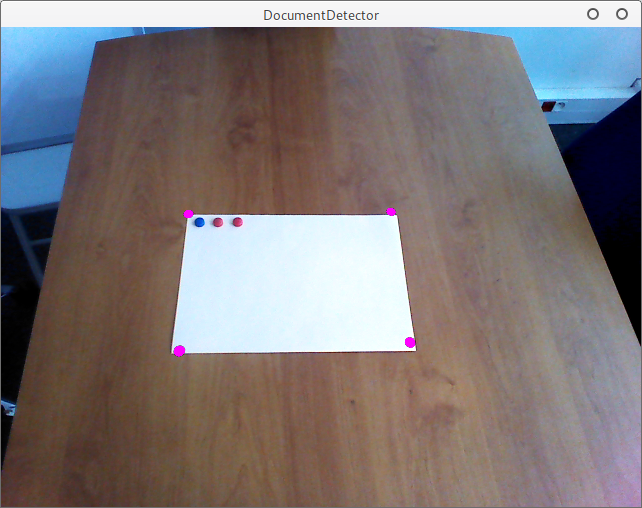
\includegraphics[width=0.5\textwidth]{images/document-detection-simple}
      \label{sub:docdetect:simple}
      }
      \subfloat[Avec connaissance à priori: Taille du document et distance élément $\longleftrightarrow$ coin]{
      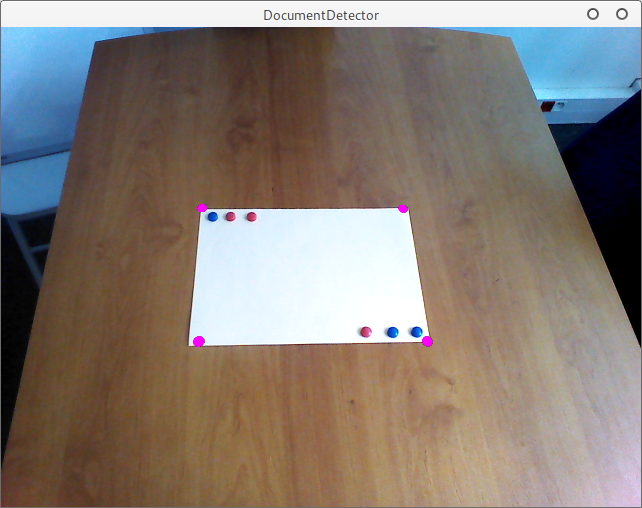
\includegraphics[width=0.5\textwidth]{images/document-detection-double}
      \label{sub:docdetect:double}
      }\\
      \subfloat[Avec connaissance à priori: Taille du document]{
      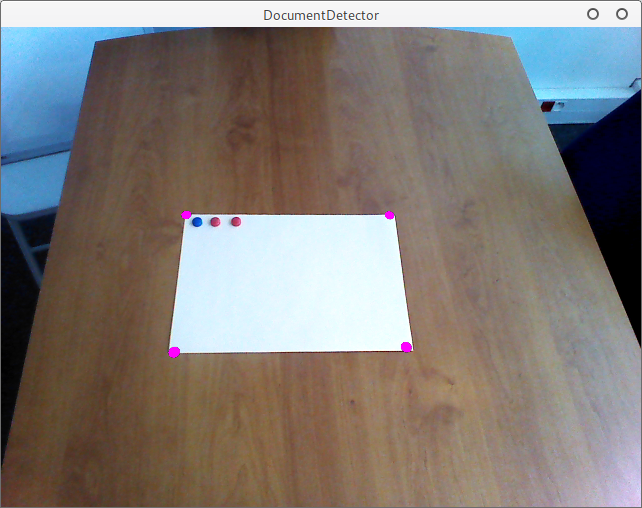
\includegraphics[width=0.5\textwidth]{images/document-detection-corner}
      \label{sub:docdetect:corner}
      }
      \subfloat[Sans connaissance à priori]{
      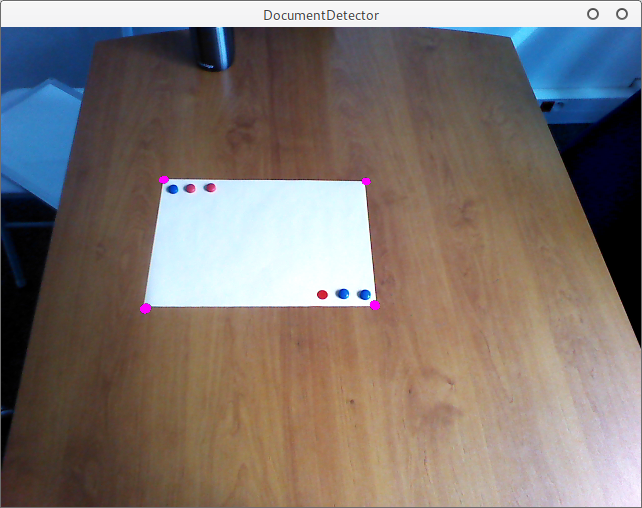
\includegraphics[width=0.5\textwidth]{images/document-detection-double-corner}
      \label{sub:docdetect:double-corner}
      }
      \caption{Résultats des différentes versions de la détection de document.}
      \label{fig:docdetect:results}
\end{figure}
